% !TEX root = ../main.tex
\chapter{THỰC NGHIỆM VÀ ĐÁNH GIÁ}
\label{chap:evaluation}

\section{Mục tiêu và thiết lập thực nghiệm}
\label{sec:evaluation-setup}

\subsection{Mục tiêu và phạm vi đánh giá}

Thực nghiệm được xây dựng nhằm đánh giá khả năng điều khiển cân bằng của quadrotor sau khi tích hợp phần cứng và chương trình trên STM32. Ba nội dung khảo sát gồm duy trì tư thế gần nằm ngang, bám các thay đổi nhỏ của góc đặt và trở về tư thế mong muốn sau tác động gây lệch. Kết quả được xem xét qua diễn biến góc, vận tốc góc và lệnh động cơ, kết hợp với các chỉ tiêu định lượng để mô tả sai lệch và mức dao động của hệ thống.

Quá trình đánh giá gồm hai giai đoạn: thử nghiệm trên bộ gá gimbal và thử nghiệm bay thực tế. Bộ gá tạo điều kiện khảo sát chuyển động quay trong khi vị trí của mô hình được giữ bởi kết cấu cơ khí, phục vụ hiệu chỉnh và lựa chọn tham số điều khiển. Thử nghiệm bay tiếp tục đánh giá đáp ứng tư thế khi quadrotor rời bộ gá. Phạm vi phân tích tập trung vào hai góc roll $\phi$ và pitch $\theta$ gần tư thế nằm ngang; độ cao, vị trí và chuyển động yaw được mô tả như điều kiện vận hành khi có dữ liệu tương ứng.

\subsection{Mô hình và bố trí thực nghiệm}

Mô hình sử dụng phần cứng đã trình bày trong \charef{chap:system-design}, gồm khung F450, bốn cụm động cơ--ESC--cánh quạt, nguồn pin LiPo 3S và bo điều khiển STM32F103VET6. Cảm biến quán tính cung cấp tín hiệu phản hồi, còn bộ thu ELRS tiếp nhận lệnh từ tay điều khiển Jumper T20 V2. Hai dạng bộ gá được sử dụng để phục vụ các nội dung kiểm tra khác nhau: gimbal dạng trụ đứng và gimbal khung hình vuông.

Gimbal dạng trụ đứng trong \fref{fig:evaluation-stand} có phần đế bằng nhôm định hình và trụ đỡ liên kết với cụm trung tâm của quadrotor. Bốn tay đòn cùng các động cơ nằm phía ngoài trụ, thuận tiện cho việc quan sát thân máy bay, tiếp cận bo mạch và kiểm tra dây nối. Cách bố trí này phù hợp với giai đoạn kiểm tra tích hợp, khi cần đối chiếu trực tiếp chuyển động của mô hình với tín hiệu phản hồi và tác động điều khiển.

\begin{figure}[H]
	\centering
	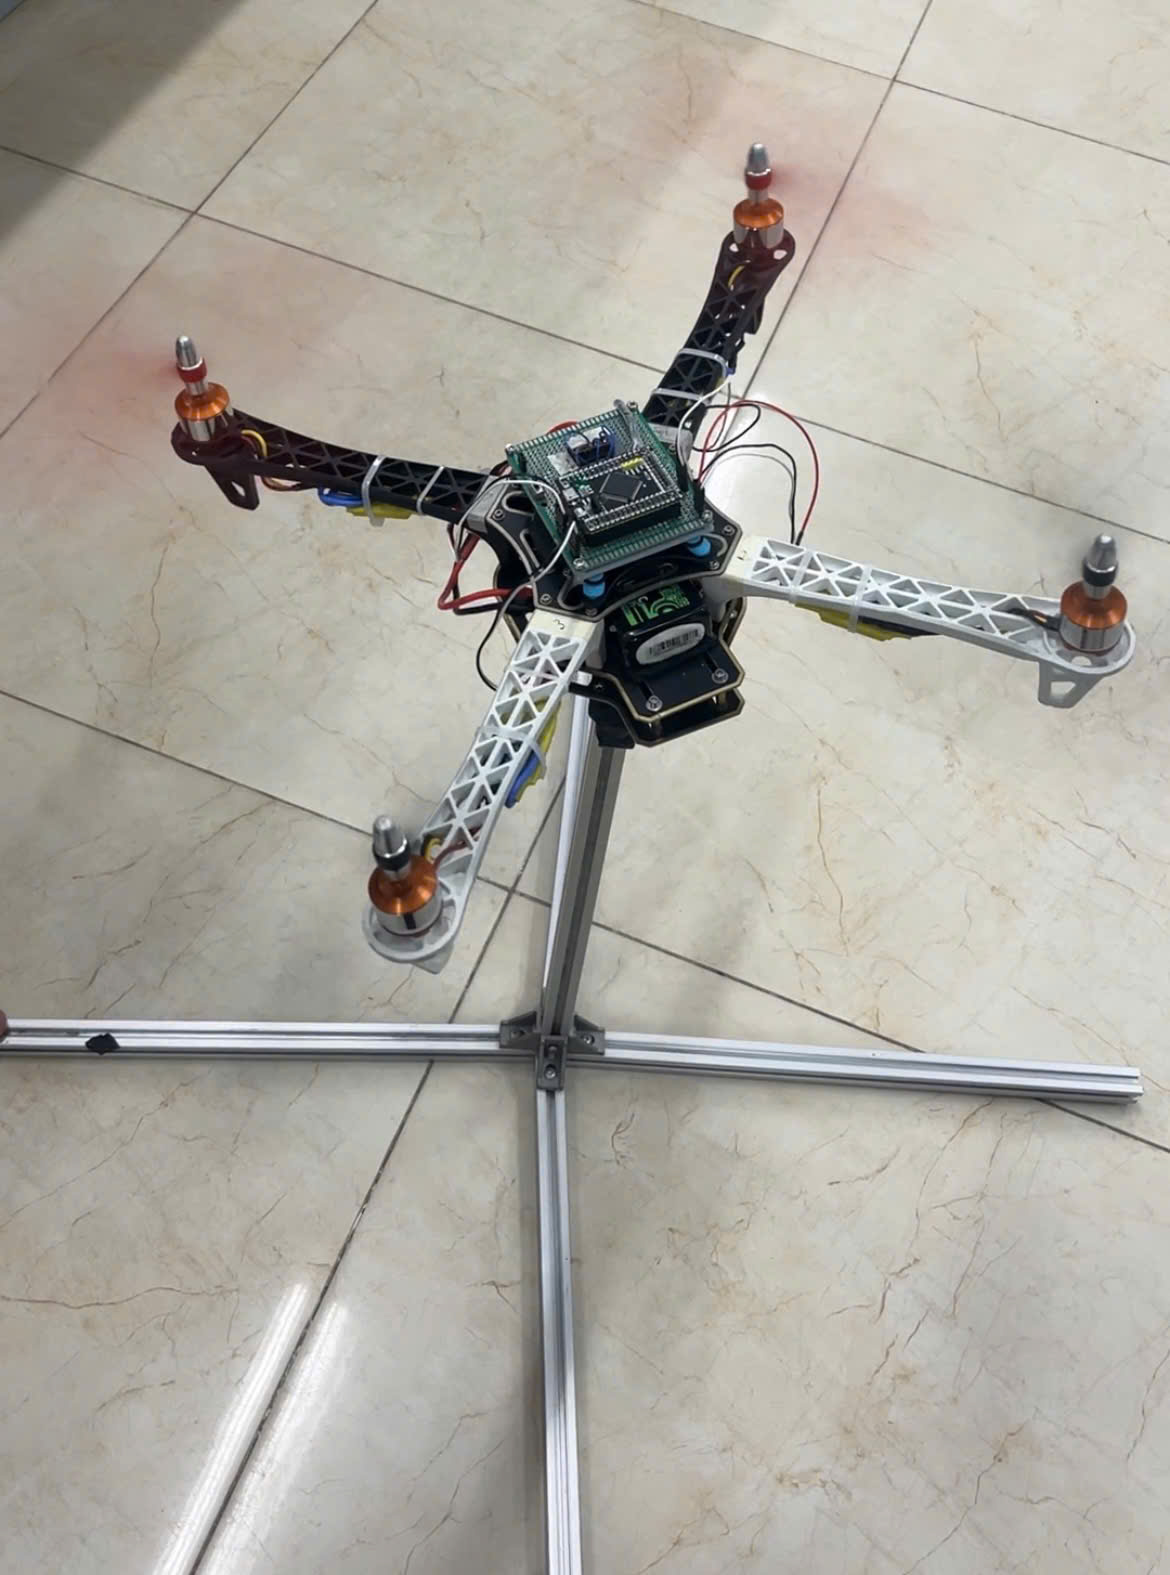
\includegraphics[height=8.5cm,width=0.75\linewidth,keepaspectratio]{figures/ch04/gimbal-stand.jpg}
	\caption{Mô hình quadrotor trên bộ gá gimbal dạng trụ đứng.}
	\label{fig:evaluation-stand}
\end{figure}

Nội dung kiểm tra đầu tiên trên gimbal trụ đứng là sự tương ứng giữa chiều nghiêng của thân và tín hiệu cảm biến. Khi nghiêng mô hình theo chiều roll hoặc pitch dương, góc ước lượng và vận tốc góc phản hồi được đối chiếu với quy ước hệ trục thân. Phép kiểm tra này giúp nhận biết sai thứ tự trục, sai dấu hoặc sai hướng lắp cảm biến trước khi hiệu chỉnh bộ điều khiển. Tiếp theo, phản ứng của các cặp động cơ được xem xét để xác định mômen hiệu chỉnh có hướng đưa thân về tư thế đặt hay làm tăng độ lệch.

Khi các trục khảo sát được liên kết cho phép quay, gimbal trụ đứng còn phục vụ đánh giá sơ bộ khả năng tự cân bằng. Với góc đặt roll và pitch bằng không, mô hình được tạo một độ lệch nhỏ rồi thả để quan sát xu hướng trở về nằm ngang, dao động và ảnh hưởng qua lại giữa hai kênh. Ưu điểm của bố trí này là dễ quan sát đồng thời chuyển động thân và phản ứng của bốn cụm động cơ, phù hợp để phát hiện lỗi tích hợp và lựa chọn bộ tham số điều khiển ban đầu.

Gimbal khung hình vuông trong \fref{fig:evaluation-gimbal} được lắp từ các thanh nhôm định hình, với mô hình bố trí ở vùng giữa khung và các liên kết quay đặt ở hai phía đối diện. Khung ngoài làm giá đỡ, còn các liên kết quay xác định hướng chuyển động của phần gá mang quadrotor. Bố trí này phù hợp với các phép thử có trục quay xác định, giúp tập trung khảo sát đáp ứng của từng kênh điều khiển.

\begin{figure}[H]
	\centering
	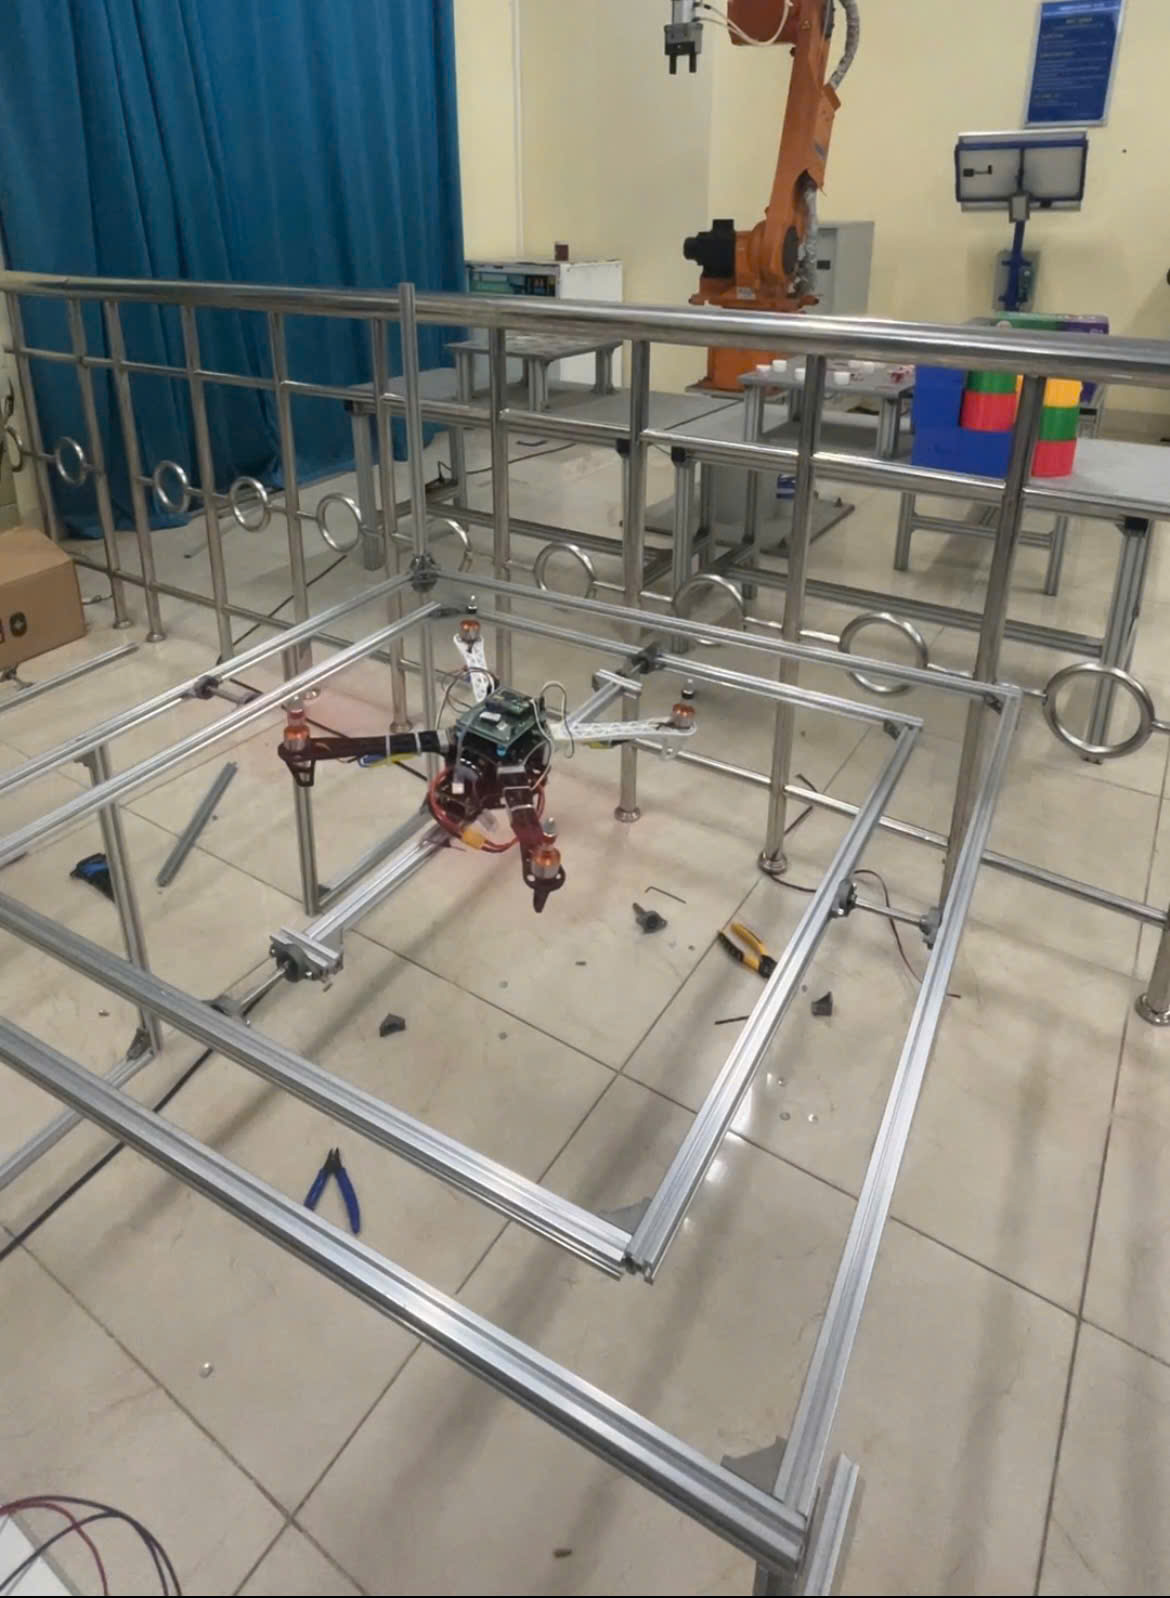
\includegraphics[height=8.5cm,width=0.75\linewidth,keepaspectratio]{figures/ch04/gimbal-frame.jpg}
	\caption{Mô hình quadrotor trên bộ gá gimbal khung hình vuông.}
	\label{fig:evaluation-gimbal}
\end{figure}

Để khảo sát riêng roll hoặc pitch, trục quay của bộ gá được bố trí trùng với trục thân tương ứng, đồng thời các chuyển động còn lại được hạn chế theo cấu hình gá. Trên cấu hình này, vòng vận tốc góc được khảo sát trước thông qua khả năng bám lệnh và mức dao động của vận tốc phản hồi. Sau khi lựa chọn tham số vòng trong, vòng góc được đánh giá bằng các thay đổi nhỏ của góc đặt để quan sát tốc độ đáp ứng, xu hướng vượt góc đặt và khả năng duy trì tư thế. Cách khảo sát từng trục giúp phân biệt rõ ảnh hưởng của tham số điều khiển roll và pitch.

Gimbal khung hình vuông cũng phù hợp với phép thử phục hồi sau nhiễu: giữ góc đặt không đổi, tạo độ lệch nhỏ quanh trục khảo sát rồi theo dõi quá trình trở lại tư thế đặt. Các lượt so sánh tham số sử dụng cùng cấu hình gá, mức ga và dạng tác động để làm rõ sự thay đổi của đáp ứng. Khi khảo sát liên kết giữa roll và pitch, bộ gá được cấu hình cho phép hai chuyển động này; phản hồi của cả hai kênh được quan sát đồng thời để đánh giá khả năng phối hợp điều khiển.

Với cả hai dạng gimbal, vị trí pin, bo mạch và dây dẫn được giữ ổn định giữa các lượt so sánh. Vị trí trục đỡ so với trọng tâm, ma sát tại liên kết quay và quán tính của phần gá chuyển động đều ảnh hưởng đến đáp ứng. Vì vậy, kết quả trên bộ gá được diễn giải theo điều kiện cơ khí tương ứng và dùng làm cơ sở lựa chọn tham số trước khi đánh giá tiếp bằng thử nghiệm bay thực tế.
